\documentclass{article}
\usepackage{graphicx} % new way of doing eps files
\usepackage{listings} % nice code layout
\usepackage[usenames]{color} % color
\definecolor{listinggray}{gray}{0.9}
\definecolor{graphgray}{gray}{0.7}
\definecolor{ans}{rgb}{1,0,0}
\definecolor{blue}{rgb}{0,0,1}
% \Verilog{title}{label}{file}
\newcommand{\Verilog}[3]{
  \lstset{language=Verilog}
  \lstset{backgroundcolor=\color{listinggray},rulecolor=\color{blue}}
  \lstset{linewidth=\textwidth}
  \lstset{commentstyle=\textit, stringstyle=\upshape,showspaces=false}
  \lstset{frame=tb}
  \lstinputlisting[caption={#1},label={#2}]{#3}
}


\author{your names}
\title{Lab title}

\begin{document}
\maketitle

\section{Introduction}
Introduction with problem overview, your design procedure, and rationale.  Be as brief as possible to let me know the big picture of the lab.

\section{Interface}
Since we have already shown our inputs and outputs for the non-pipelined datapath, there is no need to detail every input and output again.  Therefore, you can leave this section blank.  

\section{Design}
This section should show your pipeline analysis spreadsheet where we showed the contents of the pipeline buffers.  If you can display it in a readable way in this document, then please do so.  Otherwise, include the document or an image of the document in your Git repository and point to that document (it does not have to be a link, just a description of where it is in your repository).

\section{Implementation}
Show your Verilog code that is pertinent to pipelining.  This should include (but is not limited to) datapath.v, iFetch.v, iDecode.v, iExecute.v, iMemory.v, and iWriteBack.v.  Code should be included in the report like Listing~\ref{code:reg} on page~\pageref{code:reg}. 

\Verilog{Verilog code for implementing a register.}{code:reg}{../code/1_fetch/register.v}

\section{Test}
This is where you should show the code you used to test your pipeline and the results.  Please include:
\begin{enumerate}
	\item List of assembly commands that you used to test your pipeline
	\item Binary for the commands you have been using to test your datapath since the iDecode stage
	\item Simulation Results from these commands.  Please make sure that I can see all values in the table.  This might be difficult, as there are a lot of signals.  You can use multiple diagrams if necessary.  A sample simulation diagram is in Figure~\ref{fig:regtest} on page~\pageref{fig:regtest}.
\end{enumerate}

\Verilog{Verilog code for testing a register.}{code:regtest}{../code/1_fetch/register_test.v}

\begin{figure}
\begin{center}
\caption{Timing diagram for the register test.}\label{fig:regtest}
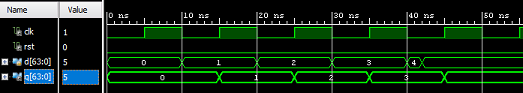
\includegraphics[width=0.9\textwidth]{../images/registertiming.png}
\end{center}
\end{figure}

\section{Conclusions}
Describe the behavior you achieved in your pipeline.  Did it work correctly?  How long did it take to execute?  How long would it take on a non-pipelined datapath?  Can you make it run faster by reducing the cycle time?  What can be done in future labs to make it run faster?
\end{document} 